\subsection{package kit.edu.pse.fridget.client.activity}
\begin{figure}[H]
	       \centering
	       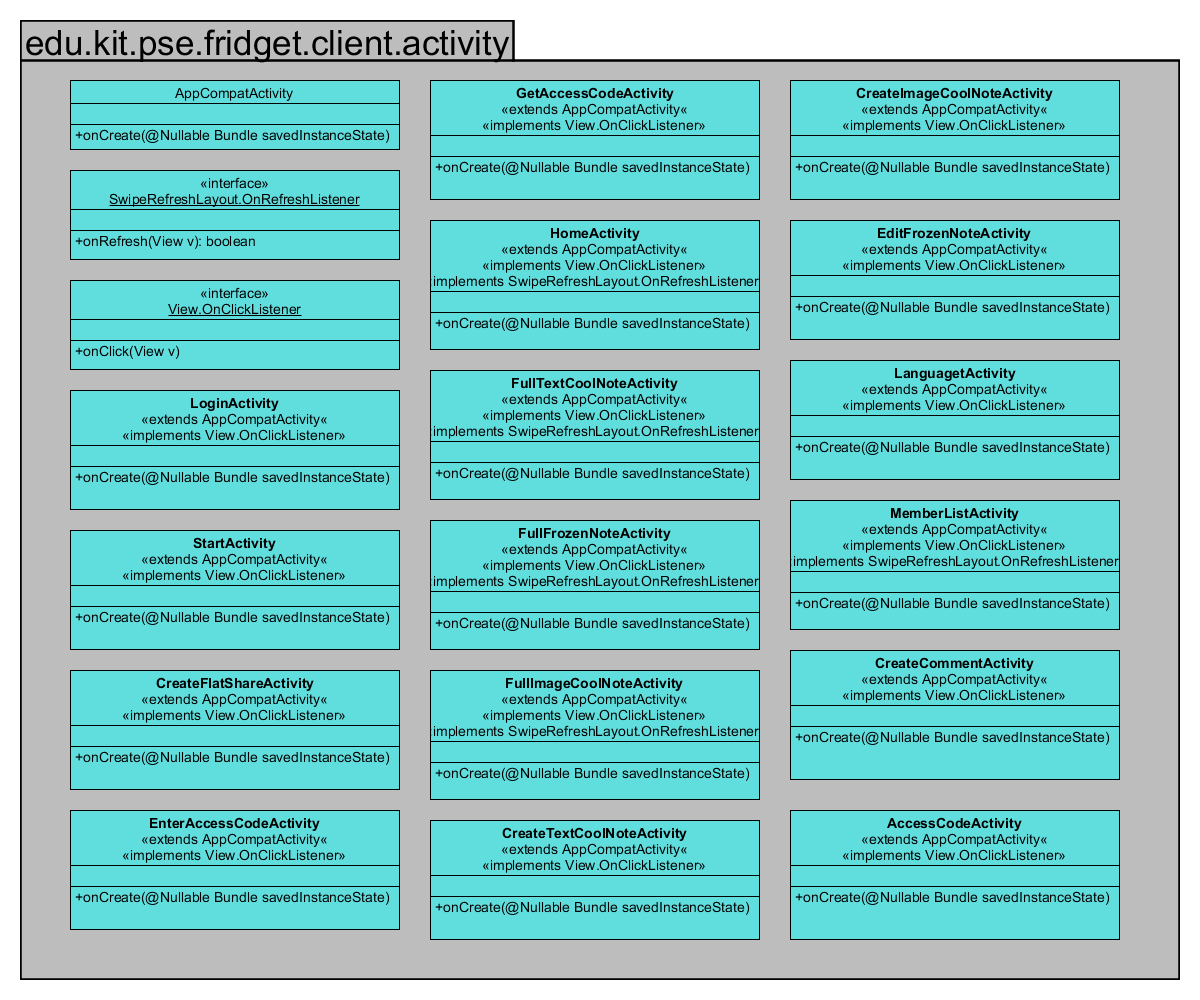
\includegraphics[scale = .35]{klassendiagramm_activity.png}
	       \caption{Klassen der Activities}
	      \end{figure}
\subsubsection{\texttt{public class AppCompatActivity}}

	\textbf{Beschreibung} \\
	\textit{Basisklasse für alle Activities} \\

	\textbf{Methoden}
	\begin{itemize}
		\item{\texttt{public void onCreate(@Nullable Bundle savedInstanceState)}}\\
	\textit{Hier wird das Layout der Activity erstellt.}\\
	\end{itemize}

	\textbf{Parameter}
	\begin{itemize}
		\item\texttt{Bundle savedInstanceState}\\ 
	\textit{Die zuvor gespeicherte Instanz der Activity, die wieder hergestellt zwird, sonst NULL}\\
	\end{itemize}

\subsubsection{\texttt{public static interface View.OnClickListener}}

	\textbf{Beschreibung} \\
	\textit{Schnittstelle dafür, wenn auf die View geklickt wird.klickt wird.}\\

	\textbf{Methoden}
	\begin{itemize}
	\item{\texttt{public void onClick(View v)}}\\
	\textit{Aufruf bei einen Klick auf ein Element.}\\
	\end{itemize}

	\textbf{Parameter}
	\begin{itemize}
	\item\texttt{View v}\\
	\textit{Die angeklickte View}\\
	\end{itemize} 

\subsubsection{\texttt{public static interface SwipeRefreshLayout.OnRefreshListener}}

	\textbf{Beschreibung} \\
	\textit{Schnittstelle dafür, wenn durch Hinunter-Swipen eine Aktualisierung ausgeführt werden soll} \\

	\textbf{Methoden}
	\begin{itemize}
		\item\texttt{{public boolean onRefresh()}}\\
	\textit{Aufruf beim Hinunter-Swipen zum Aktualisieren}\\
	\end{itemize}       

\subsubsection{\texttt{public class LoginActivity extends AppCompatActivity implements View.OnClickListener}}

	\textbf{Beschreibung} \\
	\textit{Diese Klasse zeigt den Login mit dem Google-Account. Man kann seinen Google-Account-Daten eingeben und sich anmelden.} \\

	\textbf{Methoden}
	\begin{itemize}
		\item\texttt{{public void onCreate(@Nullable Bundle savedInstanceState)}}\\
	\textit{Hier wird das Layout der Activity erstellt.}\\
	\end{itemize}

	\textbf{Parameter}
	\begin{itemize}
		\item\texttt{Bundle savedInstanceState}\\ 
	\textit{Die zuvor gespeicherte Instanz der Activity, die wieder hergestellt zwird, sonst NULL}\\
	\end{itemize}

\subsubsection{\texttt{public class StartActivity extends AppCompatActivity implements View.OnClickListener}}

	\textbf{Beschreibung} \\
	\textit{Diese Klasse zeigt den Startbildschirm mit dem App-Logo und zwei Buttons: Ein Button zum Erstellen einer WG und einer zum Eingeben eines Zugangscodes.} \\

	\textbf{Methoden}
	\begin{itemize}
		\item\texttt{{public void onCreate(@Nullable Bundle savedInstanceState)}}\\
	\textit{Hier wird das Layout der Activity erstellt.}\\
	\end{itemize}

	\textbf{Parameter}
	\begin{itemize}
		\item\texttt{Bundle savedInstanceState}\\ 
	\textit{Die zuvor gespeicherte Instanz der Activity, die wieder hergestellt zwird, sonst NULL}\\
	\end{itemize}       

\subsubsection{\texttt{public class CreateFlatshareActivity extends AppCompatActivity implements View.OnClickListener}}

	\textbf{Beschreibung} \\
	\textit{In dieser Klasse kann man der WG einen Namen geben und kann mithilfe eines Buttons zur HomeActivity gelangen.} \\

	\textbf{Methoden}
	\begin{itemize}
		\item\texttt{{public void onCreate(@Nullable Bundle savedInstanceState)}}\\
	\textit{Hier wird das Layout der Activity erstellt.}\\
	\end{itemize}

	\textbf{Parameter}
	\begin{itemize}
		\item\texttt{Bundle savedInstanceState}\\ 
	\textit{Die zuvor gespeicherte Instanz der Activity, die wieder hergestellt zwird, sonst NULL}\\
	\end{itemize}      

\subsubsection{\texttt{public class GetAccessCodeActivity extends AppCompatActivity implements View.OnClickListener}}

	\textbf{Beschreibung} \\
	\textit{In dieser Klasse kriegt man den Zugangscode und kann mithilfe eines Buttons zur HomeActivity gelangen.} \\

	\textbf{Methoden}
	\begin{itemize}
		\item\texttt{{public void onCreate(@Nullable Bundle savedInstanceState)}}\\
	\textit{Hier wird das Layout der Activity erstellt.}\\
	\end{itemize}

	\textbf{Parameter}
	\begin{itemize}
		\item\texttt{Bundle savedInstanceState}\\  
	\textit{Die zuvor gespeicherte Instanz der Activity, die wieder hergestellt zwird, sonst NULL}\\
	\end{itemize}  

\subsubsection{\texttt{public class EnterAccessCodeActivity extends AppCompatActivity implements View.OnClickListener}}

	\textbf{Beschreibung} \\
	\textit{In dieser Klasse kann man den Zugangscode eingeben und kann mithilfe eines Buttons zur HomeActivity gelangen.} \\

	\textbf{Methoden}
	\begin{itemize}
		\item\texttt{{public void onCreate(@Nullable Bundle savedInstanceState)}}\\
	\textit{Hier wird das Layout der Activity erstellt.}\\
	\end{itemize}

	\textbf{Parameter}
	\begin{itemize}
		\item\texttt{Bundle savedInstanceState}\\ 
	\textit{Die zuvor gespeicherte Instanz der Activity, die wieder hergestellt zwird, sonst NULL}\\
	\end{itemize} 

\subsubsection{\texttt{public class HomeActivity extends AppCompatActivity implements View.OnClickListener implements SwipeRefreshLayout.OnRefreshListener}}

	\textbf{Beschreibung} \\
	\textit{Diese Klasse zeigt das View der WG-Pinnwand, man sieht die Notes mit Überschrift und Magnet und einige Buttons. Drei Frozen Notes sind von Anfang an enthalten. Frozen Notes haben immer einen schwarzen Magneten.} \\

	\textbf{Methoden}
	\begin{itemize}
		\item\texttt{{public void onCreate(@Nullable Bundle savedInstanceState)}}\\
	\textit{Hier wird das Layout der Activity erstellt.}\\
	\end{itemize}

	\textbf{Parameter}
	\begin{itemize}
		\item\texttt{Bundle savedInstanceState}\\  
	\textit{Die zuvor gespeicherte Instanz der Activity, die wieder hergestellt zwird, sonst NULL}\\
	\end{itemize} 

\subsubsection{\texttt{public class FullTextCoolNoteActivity extends AppCompatActivity implements View.OnClickListener implements SwipeRefreshLayout.OnRefreshListener}}

	\textbf{Beschreibung} \\
	\textit{Diese Klasse zeigt eine Großansicht einer Text-Cool-Note mit zugehörigem Magneten, Erstelldatum, Tags, Titel, Inhalt, Lesebestätigungen und Kommentaren. Der @All-Tag ist immer da, wenn keine Tags spezifiziert werden. Es stehen wieder einige Buttons zur Interaktion zu Verfügung.} \\

	\textbf{Methoden}
	\begin{itemize}
		\item\texttt{{public void onCreate(@Nullable Bundle savedInstanceState)}}\\
	\textit{Hier wird das Layout der Activity erstellt.}\\
	\end{itemize}

	\textbf{Parameter}
	\begin{itemize}
		\item\texttt{Bundle savedInstanceState}\\ 
	\textit{Die zuvor gespeicherte Instanz der Activity, die wieder hergestellt zwird, sonst NULL}\\
	\end{itemize} 

\subsubsection{\texttt{public class FullFrozenNoteActivity extends AppCompatActivity implements View.OnClickListener implements SwipeRefreshLayout.OnRefreshListener}}

	\textbf{Beschreibung} \\
	\textit{Diese Klasse zeigt eine Großansicht einer Frozen Note mit zugehörigem schwarzen Magneten, Titel und Inhalt. Es stehen wieder einige Buttons zur Interaktion zu Verfügung.} \\

	\textbf{Methoden}
	\begin{itemize}
		\item\texttt{{public void onCreate(@Nullable Bundle savedInstanceState)}}\\
	\textit{Hier wird das Layout der Activity erstellt.}\\
	\end{itemize}

	\textbf{Parameter}
	\begin{itemize}
		\item\texttt{Bundle savedInstanceState}\\ 
	\textit{Die zuvor gespeicherte Instanz der Activity, die wieder hergestellt zwird, sonst NULL}\\
	\end{itemize} 

\subsubsection{\texttt{public class FullImageCoolNoteActivity extends AppCompatActivity implements View.OnClickListener implements SwipeRefreshLayout.OnRefreshListener}}

	\textbf{Beschreibung} \\
	\textit{Diese Klasse zeigt eine Großansicht einer Bild-Cool-Note mit zugehörigem Magneten, Erstelldatum, Tags, Titel, Inhalt, Lesebestätigungen und Kommentaren. Der @All-Tag ist immer da, wenn keine Tags spezifiziert werden. Es stehen wieder einige Buttons zur Interaktion zu Verfügung.} \\

	\textbf{Methoden}
	\begin{itemize}
		\item\texttt{{public void onCreate(@Nullable Bundle savedInstanceState)}}\\
	\textit{Hier wird das Layout der Activity erstellt.}\\
	\end{itemize}

	\textbf{Parameter}
	\begin{itemize}
		\item\texttt{Bundle savedInstanceState}\\ 
	\textit{Die zuvor gespeicherte Instanz der Activity, die wieder hergestellt zwird, sonst NULL}\\
	\end{itemize} 

\subsubsection{\texttt{public class CreateTextCoolNoteActivity extends AppCompatActivity implements View.OnClickListener}}

	\textbf{Beschreibung} \\
	\textit{Diese Klasse zeigt das View für die Erstellung einer Text-Cool-Note. Dieses View wird auch für die Kommentar-Funktion benutzt, nur, dass man keinen Titel schreiben und keine Wichtigkeit auswählen kann. Das View öffnet sich auch, wenn man eine Frozen Note editieren will, wobei die Wichtigkeit wieder nicht auswählbar ist.} \\

	\textbf{Methoden}
	\begin{itemize}
		\item\texttt{{public void onCreate(@Nullable Bundle savedInstanceState)}}\\
	\textit{Hier wird das Layout der Activity erstellt.}\\
	\end{itemize}

	\textbf{Parameter}
	\begin{itemize}
		\item\texttt{Bundle savedInstanceState}\\  
	\textit{Die zuvor gespeicherte Instanz der Activity, die wieder hergestellt zwird, sonst NULL}\\
	\end{itemize} 


\subsubsection{\texttt{public class CreateImageCoolNoteActivity extends AppCompatActivity implements View.OnClickListener}}

	\textbf{Beschreibung} \\
	\textit{Diese Klasse zeigt das View für die Erstellung einer Bild-Cool-Note.} \\

	\textbf{Methoden}
	\begin{itemize}
		\item\texttt{{public void onCreate(@Nullable Bundle savedInstanceState)}}\\
	\textit{Hier wird das Layout der Activity erstellt.}\\
	\end{itemize}

	\textbf{Parameter}
	\begin{itemize}
		\item\texttt{Bundle savedInstanceState}\\ 
	\textit{Die zuvor gespeicherte Instanz der Activity, die wieder hergestellt zwird, sonst NULL}\\
	\end{itemize} 

\subsubsection{\texttt{public class CreateCommentActivity extends AppCompatActivity implements View.OnClickListener}}

	\textbf{Beschreibung} \\
	\textit{Diese Klasse zeigt das View für die Erstellung eines Kommentars.} \\

	\textbf{Methoden}
	\begin{itemize}
		\item\texttt{{public void onCreate(@Nullable Bundle savedInstanceState)}}\\
	\textit{Hier wird das Layout der Activity erstellt.}\\
	\end{itemize}

	\textbf{Parameter}
	\begin{itemize}
		\item\texttt{Bundle savedInstanceState}\\  
	\textit{Die zuvor gespeicherte Instanz der Activity, die wieder hergestellt zwird, sonst NULL}\\
	\end{itemize} 


\subsubsection{\texttt{public class EditFrozenNoteActivity extends AppCompatActivity implements View.OnClickListener}}

	\textbf{Beschreibung} \\
	\textit{Diese Klasse zeigt das View für die Bearbeitung einer Frozen Note.} \\

	\textbf{Methoden}
	\begin{itemize}
		\item\texttt{{public void onCreate(@Nullable Bundle savedInstanceState)}}\\
	\textit{Hier wird das Layout der Activity erstellt.}\\
	\end{itemize}

	\textbf{Parameter}
	\begin{itemize}
		\item\texttt{Bundle savedInstanceState}\\ 
	\textit{Die zuvor gespeicherte Instanz der Activity, die wieder hergestellt zwird, sonst NULL}\\
	\end{itemize} 

\subsubsection{\texttt{public class MemberListActivity extends AppCompatActivity implements View.OnClickListener implements SwipeRefreshLayout.OnRefreshListener}}

	\textbf{Beschreibung} \\
	\textit{Diese Klasse zeigt das View zum Einsehen der aktuellen Mitglieder mit
mit zugehörigem Magneten.} \\

	\textbf{Methoden}
	\begin{itemize}
		\item\texttt{{public void onCreate(@Nullable Bundle savedInstanceState)}}\\
	\textit{Hier wird das Layout der Activity erstellt.}\\
	\end{itemize}

	\textbf{Parameter}
	\begin{itemize}
		\item\texttt{Bundle savedInstanceState}\\  
	\textit{Die zuvor gespeicherte Instanz der Activity, die wieder hergestellt zwird, sonst NULL}\\
	\end{itemize} 

\subsubsection{\texttt{public class LanguageActivity extends AppCompatActivity implements View.OnClickListener}}

	\textbf{Beschreibung} \\
	\textit{Diese Klasse zeigt das View zum Einstellen der App-Sprache.} \\

	\textbf{Methoden}
	\begin{itemize}
		\item\texttt{{public void onCreate(@Nullable Bundle savedInstanceState)}}\\
	\textit{Hier wird das Layout der Activity erstellt.}\\
	\end{itemize}

	\textbf{Parameter}
	\begin{itemize}
		\item\texttt{Bundle savedInstanceState}\\  
	\textit{Die zuvor gespeicherte Instanz der Activity, die wieder hergestellt zwird, sonst NULL}\\
	\end{itemize} 

\subsubsection{\texttt{public class AccessCodeActivity extends AppCompatActivity implements View.OnClickListener}}

\textbf{Beschreibung} \\
\textit{Diese Klasse zeigt das View zum Erstellen eines neuen Zugangscodes.} \\

\textbf{Methoden}
\begin{itemize}
	\item\texttt{{public void onCreate(@Nullable Bundle savedInstanceState)}}\\
	\textit{Hier wird das Layout der Activity erstellt.}\\
\end{itemize}

\textbf{Parameter}
\begin{itemize}
	\item\texttt{Bundle savedInstanceState}\\  
	\textit{Die zuvor gespeicherte Instanz der Activity, die wieder hergestellt zwird, sonst NULL}\\
\end{itemize} 

\newpage
